\documentclass[a4paper,oneside]{article} % oneside for single page print
\usepackage[landscape,twocolumn,margin=1.5cm]{geometry}
\setlength{\columnsep}{1cm}
\usepackage{etoolbox}

\usepackage[T1]{fontenc}
\usepackage{graphicx} % for image support.
\usepackage{float} % for H option on image import

\usepackage[utf8x]{inputenc} % for utf-8 support force with: ⛺
\usepackage[usenames,dvipsnames]{color} % for color support
\usepackage{inconsolata}

\usepackage{etoolbox} % for conditionals and boolean operations on them
\usepackage{booktabs} % for table h lines
% \usepackage{a4wide}

% Math specific libraries
\usepackage{amsmath,amsfonts,amssymb} % assymb for more math symbols
\usepackage{wasysym} % For contradiction symbol \lightning
\usepackage{mathtools}
\usepackage{systeme}
\usepackage{circuitikz} % for logic circuits

\usepackage{cancel} % for the cancel command
\usepackage{rotating} % for rotating tables NOTE: Add [figuresleft] or [figuresright] so it doesn't auto-rotate
\usepackage{listings}
% \usepackage{quotchap} % for books to have quotes
\usepackage{dirtytalk} % for quick quotes with \say
\usepackage{manfnt} % for dangerous bend symbol, see: https://math.uoregon.edu/wp-content/uploads/2014/12/compsymb-1qyb3zd.pdf or use \textdbend

\usepackage{subfiles}


% Non-default packages
\usepackage{fitch}
\usepackage{bussproofs}


\lstset{language=C++,
	columns=fullflexible,
	basicstyle=\ttfamily,
	keywordstyle=\color{black}\ttfamily,
	stringstyle=\color{black}\ttfamily,
	commentstyle=\color{black}\ttfamily,
	morecomment=[l][\color{black}]{\#},
	tabsize=4,
	extendedchars=true,
	literate=%
	{Ä}{{\"A}}1%
	{Ö}{{\"O}}1%
	{Ü}{{\"U}}1%
	{ä}{{\"a}}1%
	{ö}{{\"o}}1%
	{ü}{{\"u}}1%
	{ß}{{\ss}}1%
	{←}{{:=}}1%
	{≥}{{>=}}1%
	{∧}{{$\wedge$}}1%
}


\usepackage{enumitem} % for style in \begin{description}[style=unboxed]
\usepackage[acronym]{glossaries} % alternative use glossaries
\usepackage[normalem]{ulem} % for strike-through using \sout{text to strike through}

%\usepackage[graphviz]

% Non-default packages
% \usepackage{fitch}
% \usepackage{bussproofs}

%\makeglossaries
%\input{glossary.tex}

% custom settings
\setcounter{secnumdepth}{3} % For enabling \ref to subsubsections 
% custom functions
\newcommand{\bnl}{\\ \noindent}
% Add a column with any length. Add [t] to align it on top! Reference: http://tex.stackexchange.com/questions/2441/how-to-add-a-forced-line-break-inside-a-table-cell
\newcommand{\specialcell}[2][c]{%
\begin{tabular}[#1]{@{}l@{}}#2\end{tabular}}

\newcommand{\smath}[1]{ {\setlength{\mathindent}{0cm} \begin{equation} #1\end{equation}}%
}

% MAKE ABS AND NORM GROW WHEN FRAC
\DeclarePairedDelimiter\abs{\lvert}{\rvert}%
\DeclarePairedDelimiter\norm{\lVert}{\rVert}%
% Swap the definition of \abs* and \norm*, so that \abs
% and \norm resizes the size of the brackets, and the 
% starred version does not.
\makeatletter
\let\oldabs\abs
\def\abs{\@ifstar{\oldabs}{\oldabs*}}
%
\let\oldnorm\norm
\def\norm{\@ifstar{\oldnorm}{\oldnorm*}}
\makeatother

%%%%%%%%%%%%%%%%%%
% BEGIN DOCUMENT %
%%%%%%%%%%%%%%%%%%
\begin{document}
	% initialize settings
	\pagenumbering{arabic}

	\title{Provability modal logic - George Boolos}
	\date{\today}
	\author{Kevin De Keyser}

	% title, abstract, table of contents & others
	\maketitle
	
	Zuerst sollte man zwischen der Sprache der Aussgagenlogik, der Sprache der Urteile, der Sprache der hypothetischen Urteile und der Sprache der Beweise unterscheiden.
	
	\begin{description}
	\item[Sprache der Logik] $\mathcal{L}_{modal} :=$ Formale Sprache aller (wohl-geformten) Formeln der Modellogik über das Alphabet $\Sigma_{modal} = \{\square,\bot,\rightarrow,(,)\}$ \\
		Diese können \textbf{induktiv definiert} werden:
	\begin{itemize}
		\item $\bot$ ist eine logische Formel.
		\item Alle kleingeschriebenen lateinische Charakter sind logische Formeln.
		\item Falls $\phi, \psi$ logische Formeln sind, dann sind es auch $(\phi \rightarrow \psi)$.
		\item Falls $\phi$ eine logische Formel ist, dann ist es auch $(\square \phi)$.
	\end{itemize}

	Die Sprache kann erweitert werden mit syntaktischem Zucker, wobei für alle logische Formeln $\phi,\psi$ gilt, dass folgende Formeln syntaktisch äquivalent in die rechte umgeformt werden:
	\begin{itemize}
	\item $\neg \phi :\equiv (\phi \rightarrow \bot)$
	\item $(\phi \vee \psi) :\equiv (\neg \phi \rightarrow \psi)$
	\item $(\phi \wedge \psi) :\equiv \neg (\phi \rightarrow \neg \psi)$
	\item $(\boxdot \phi) :\equiv ((\square \phi) \wedge \phi)$
	\end{itemize}

	Zusätzlich kommen nicht-erwähnte Umformungsregeln wenn Klammern ausgelassen werden (braucht wissen von Operatorpräzedenz und Assoziativität), zum Beispiel:
	$a \wedge b \wedge c \rightarrow p \rightarrow q :\equiv ((a \wedge b) \wedge c) \rightarrow (p \rightarrow q)$ 
	
	\item[Sprache der Urteile]
	
	Wahrheitsurteile sind von der Form: "$\phi$ wahr" oder "$\phi$ falsch", wobei $\phi$ wieder eine beliebige logische Formel ist.
	Urteile können auch von anderer Natur sein, wie zum Beispiel "$\phi$ falsifizierbar" oder nur schon "$\phi$ syntaktisch valid".
	
	Oft wird die Wahrheit einfach weggelassen.
	
	\item[Sprache der hypothetischen Urteile]
	Ein Sequenz (mit nur einem Konsequens) ist einfach von der Form: 
	"$\Gamma \vdash J$", wobei $\Gamma$ kommagetrennte Urteile sind (der Antedezens) und $J$ ein einzelnes Urteil ist.
	
	Es bedeutet so viel, dass wenn man die Urteile in $\Gamma$ glaubt, dann kann man aus diesen syntaktisch die Konklusion $J$ herleiten und muss somit $J$ glauben (in dieser Sprache).
	
	Zum Beispiel:
	$$\text{"}(p\rightarrow (q \rightarrow r)) \text{ wahr, } p \text{ wahr } \vdash (q \rightarrow r) \text{ wahr"}$$
	Oft lässt man hier das "wahr" weg, da herkömmliche Beweise immer über Wahrheitsurteile handeln. 
	
	Boolos verwendet selber folgende Notation (wobei $A_i,B$ logische Formeln sind):
	$<A_1,A_2,\ldots,A_n,B>$
	
	\item[Logiksystem]
	Eine Logiksystem besteht nun aus einer Menge solcher Sequenzen. Hier sind $\phi, \psi$ alles modallogische Formeln (wie zuvor induktiv definiert).
	
	\textit{Beweisregeln von GL}:
	
	Als \textbf{modus ponens} gelten alle Regeln der Form $<(\phi \rightarrow \psi),\phi,\psi>$
	
	Als \textbf{necessitation} (Notwendigkeit) gelten alle Regeln der Form $<\phi,(\square\phi)>$
	
	\textit{Axiomenschematas von GL}:
	
	Als \textbf{distribution axiom} gelten alle Regeln der Form $\vdash \square(\phi \rightarrow \psi) \rightarrow (\square \phi \rightarrow \psi)$
	
	Als \textbf{Löbs Axiom} gelten alle Regeln der Form: $\vdash \square (\square \phi \rightarrow \phi) \rightarrow \square \phi$
		
	Hinzu gelten alle Tautologien der klassichen Aussagenlogik $A$ direkt als Axiome $\vdash A$
	
	Die \textbf{Substitution} ist nicht eine explizite Regel von GL wird aber trotzdem definiert als $<F,F_p(\phi)>$, wobei $F_p(\phi)$ alle Instanzen von $p$ in $F$ durch $\phi$ ersetzt.
	
	Die \textbf{simultane Substitution} $F_{p_1,p_2,\ldots,p_n}(\phi_1,\ldots,\phi_n)$ substitutioniert alle Instanzen von $p_1,\ldots,p_n$ gleichzeitig jeweils durch $\phi_1,\ldots,\phi_n$.
	
	Sehr viele Logiker haben Fehler gemacht mit der Definition von Substitution:
	
	$(p \wedge q)_{p,q}(p \vee q, p \rightarrow q) = ((p \vee q) \wedge (p \rightarrow q))$
	$(p \wedge q)_p(p \vee q)_q(p \rightarrow q) = ((p \vee q)\wedge q)_q(p \rightarrow q) = ((p \vee (p \rightarrow q)) \wedge (p \rightarrow q))$
	
	
	\item[Sprache der Beweise] 
	Beweise kann man jetzt auf Urteilen oder hypothetischen Urteilen definieren. Dabei gibt es verschiedene Stile, solche Beweise zu machen (Gentzen, Fitch, Lemon).
	
	Eine Logik besteht aus verschiedenen Beweisregeln (wobei manche davon Axiome oder Axiomenschema sind).
	
	
	
	Gentzen's Stil (natural deduction) ist wahrscheinlich der bekannteste Stil:
	
	
	\begin{figure}[h]
	\begin{prooftree}
	\AxiomC{$L \vdash A \rightarrow B$}
	\AxiomC{}
	\RightLabel{$ax.\ nec.$}
	\UnaryInfC{$L \vdash \square (A \rightarrow B) \rightarrow ((\square A) \rightarrow (\square B))$}
	\RightLabel{$\rightarrow I$}
	\BinaryInfC{$L \vdash ((\square A) \rightarrow (\square B))$}
	\end{prooftree}
	\caption{Gentzen style proof}
	\label{fig:gentzen1}
	\end{figure}
	
	
\item[Modaloperatoren interpretieren]
	Da $\square$ ein Modaloperator über Modelformeln ist, kann dieser Operator auch als Prädikat über Formeln der Logik gedacht sein.
	
	$\square p$ in deontischer Logik wird z.B. interpretiert als: Es ist obligatorisch, dass $p$.
	
	Falls $p$ steht für Penelope drückt einen Knopf, $q$ steht für Quentin drückt einen Knopf, dann liest sich:
	$\square(p \rightarrow q) \rightarrow (\square p \rightarrow q)$ als:
	
Falls es obligatorisch ist, dass wenn Penelope einen Knopf drückt, dass dann Quentin einen Knopf drückt, dann gilt, falls es obligatorisch ist für Penelope einen Knopf zu drücken, dass das Knopfdrücken dann auch obligatorisch für Quentin ist.
 
 	In der Beweisbarkeitslogik (provability logic) gilt, dass $\square \phi$ dafür steht, dass $\phi$ beweisbar ist.
 	
 	Wir können dann für atomare Propositionen Aussagen der Peano Arithmetik anschauen wie $p \equiv (2+3=5), q \equiv 3+3=2$.
 	
 	Für solche Aussagen sieht der Satz wie folgt aus:
 	$\square(p \rightarrow q) \rightarrow (\square p \rightarrow q)$ als:



	Gödel konnte dies nur mit FOL definieren: $Bew(#p)$




	In dieser Beweisbarkeitslogik (provability logic) gilt, dass $\square \phi$ dafür steht, dass $\phi$ beweisbar ist.
		
	Nehme die Interpretation: $A(x) = x$ ist eine Gödelnummerierung einer arithmetischen Formel und diese ist wahr.
	
	Da wir nicht quantifizieren können wir gleich $p \equiv A(x)$ und $q \equiv A(y)$.
	
	Also liest sich $\square (p \rightarrow q)$ als: Es ist beweisbar, dass falls die arithmetische Aussage $x$ wahr ist, dann ist es auch die arithmetische Aussage $y$ wahr.
	
	Löbs Axiom liest sich also als:
	Falls beweisbar ist, dass wenn $\phi$ dann $\psi$, dann gilt wenn wir $\phi$ beweisen können, wir auch $\psi$ beweisen können.
	
	$\neg \square \bot$ kann gelesen werden als: Es ist unmöglich etwas falsches zu beweisen. Alternativ: Das untersuchte System ist konsistent.
	
	$\square \neq \square \bot$ sagt also aus, dass es beweisbar ist, dass das untersuchte System konsistent ist (in dem System selber). 
	
	 
	
	
	
%Fitch's Stil kommt Boolos Stil wahrscheinlich am nächsten.
%\begin{equation*}
%\begin{fitch}
%\fb (A \vee B) \rightarrow (C \wedge D) & Premise 1\\
%\fj C \rightarrow \neg D & Premise 2 \\
%\fa \neg C \vee \neg D & 2, Implication \\
%\fa \neg (C \wedge D) & 3, De Morgan's Law \\
%\fa \neg (A \vee B) & 1,4, Modens tollens \\
%\fa \neg A \wedge \neg B & 5, De Morgan's Law \\
%\fa \neg A & 6, Conjunction Elimination
%\end{fitch}
%\end{equation*}
	
	
\begin{figure}[h]
\centering
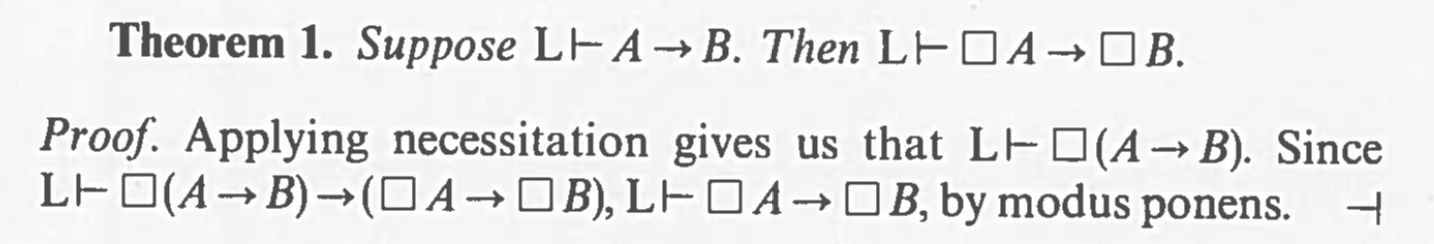
\includegraphics[width=.8\linewidth]{samplemodalproof.png}
\caption{Proof as in George Boolos text}
\label{fig:boolos1}
\end{figure}

Bei Boolos ist es vielleicht noch amüsant anzumerken, dass er ein umgekehrten Frege$\dashv \square A$

Bei Boolos ist es vielleicht noch amüsant anzumerken, dass er einen umgekehrtes turnstile verwendet um das Ende des mathematischen Arguments anzudeuten $\dashv$.





Die Sprache der Beweise ("hypothetical judgements / sequents") kann man jetzt deuten und man kann schreiben: "$p \vee q$ wahr, $p$ wahr $\vdash$ $q$ wahr".
	
	\end{description}
	
	Eine Sprache ist geschlossen, falls keine weitere ... existiert.
	
	%$\mathcal{L}_{judgement} = \{\}$

\end{document}

